%%%%%%%%%%%%%%%%%%%%%%%%%%%%%%%%%%%%%%%%%%%%%%%%%%%%%%%%%%%%%%%%%%%%%%%%%%%%%%%%
\section{Methodology}
\label{sec:meth}


\begin{figure}[]
	\centering
	\begin{subfigure}[t]{0.03\columnwidth}
	\textbf{(a)}
	\end{subfigure}
	\begin{subfigure}[t]{0.9\columnwidth}
		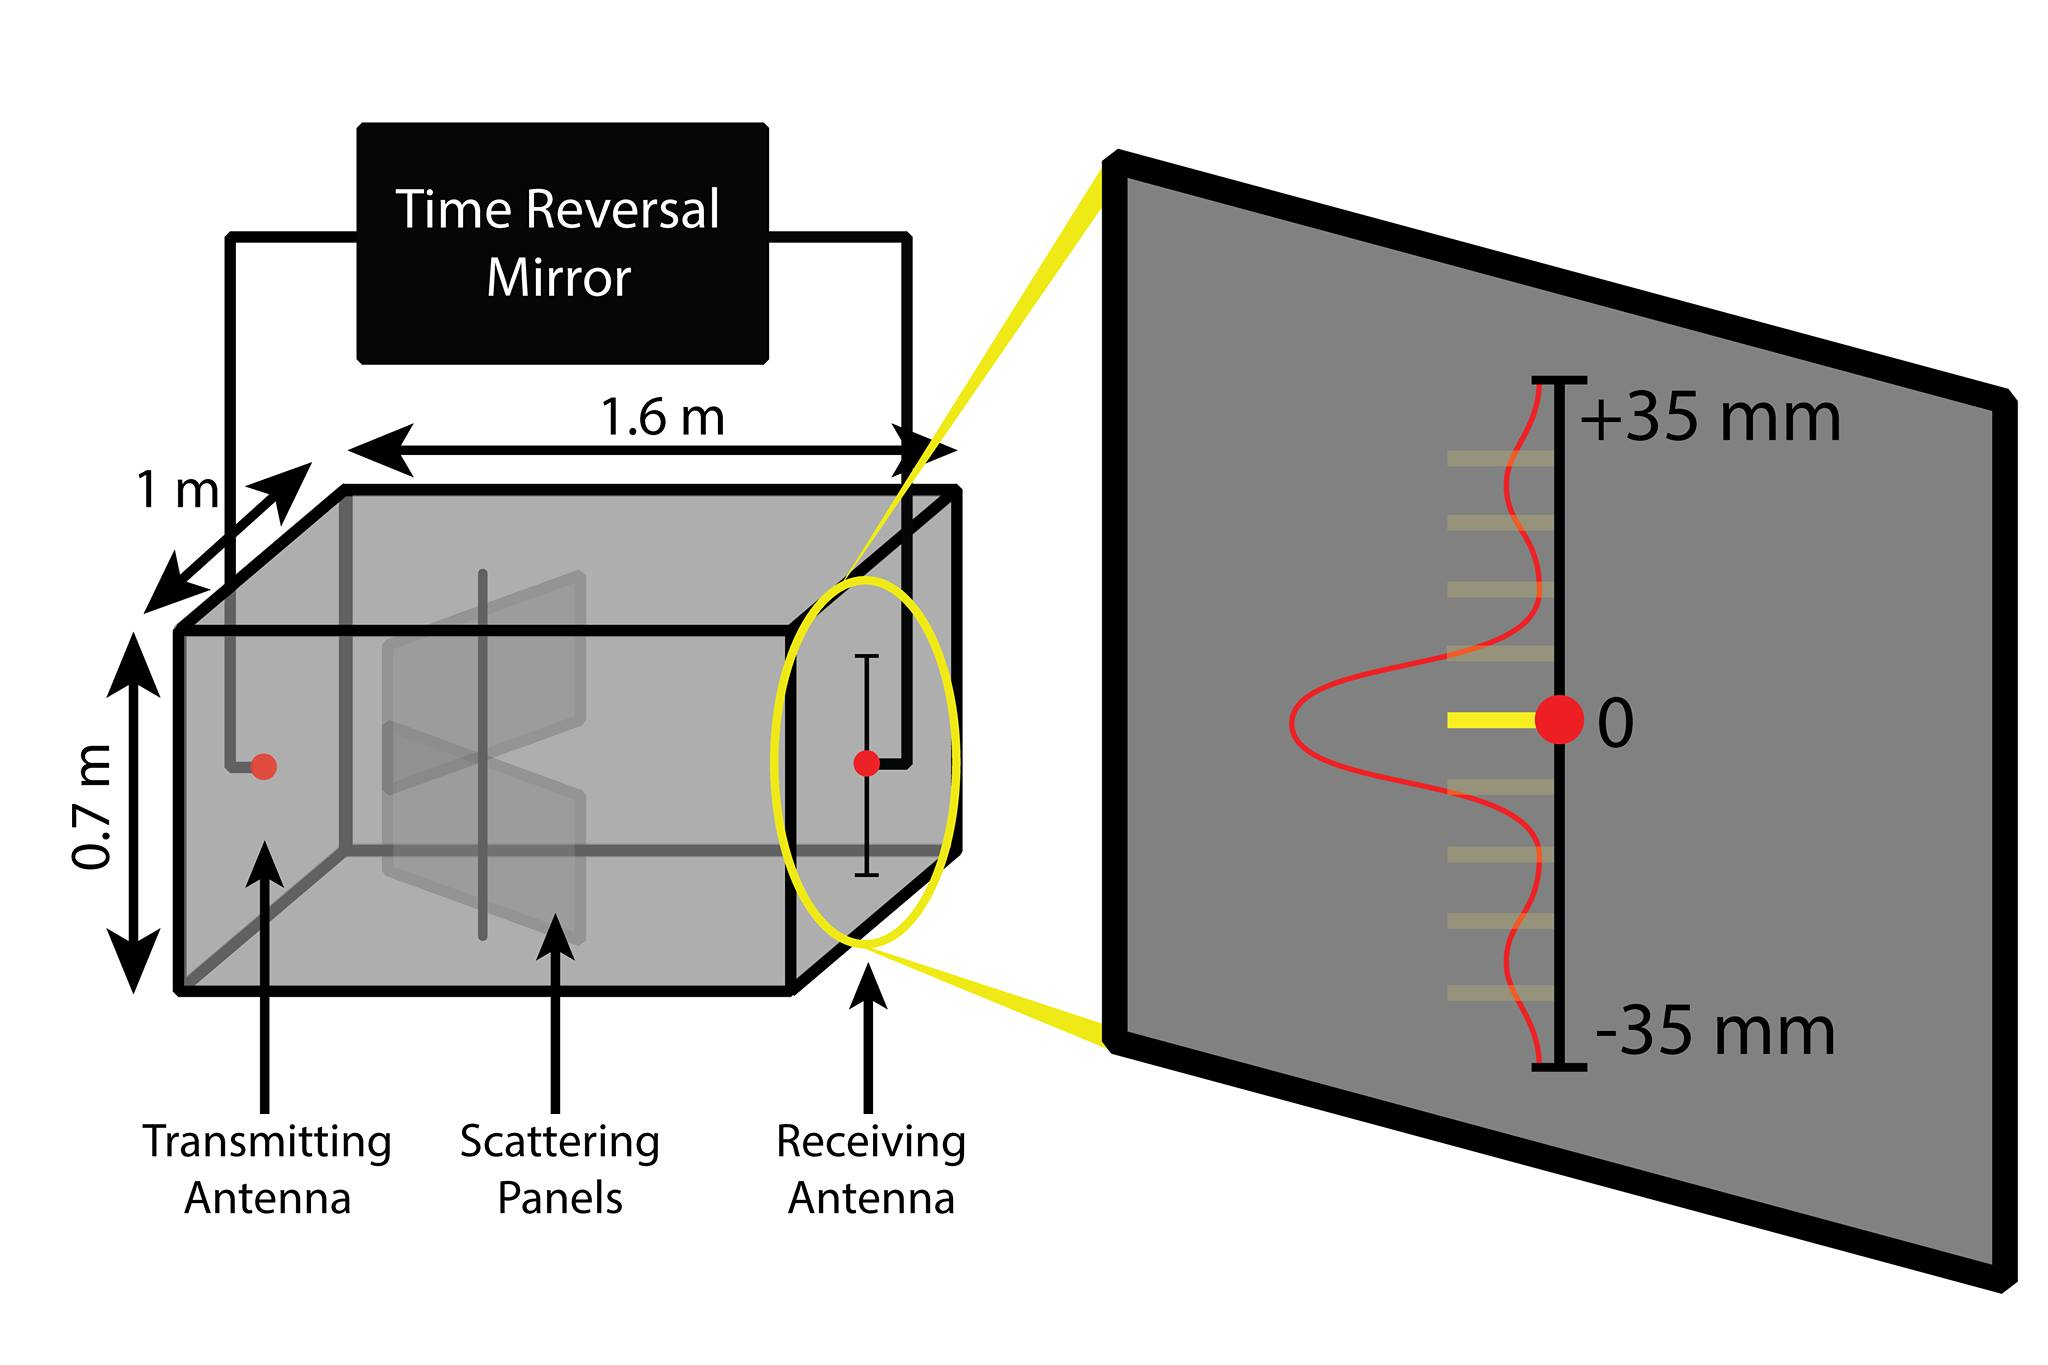
\includegraphics[width=\columnwidth,valign=t]{figs/gigabox.jpg}
		\caption{\label{fig:gigabox}}
	\end{subfigure}
	\begin{subfigure}[]{0.9\columnwidth}
		\vspace{-1.5\baselineskip}
	\begin{subfigure}[t]{0.03\columnwidth}
	\textbf{(b)}
	\end{subfigure}
		\begin{subfigure}[t]{0.45\columnwidth}
				\centering
				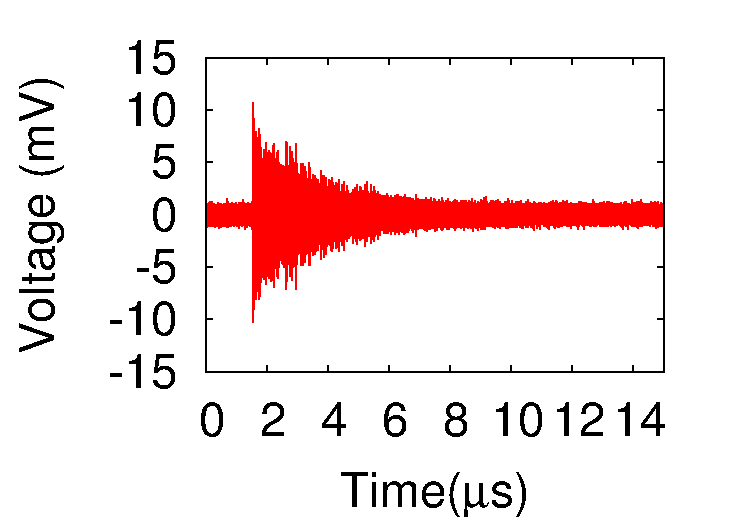
\includegraphics[width=\columnwidth,valign=t]{figs/sona.pdf}
				\caption{\label{fig:sona}}
		\end{subfigure}
	\begin{subfigure}[t]{0.03\columnwidth}
	\textbf{(c)}
	\end{subfigure}
		\begin{subfigure}[t]{0.45\columnwidth}
				\centering
				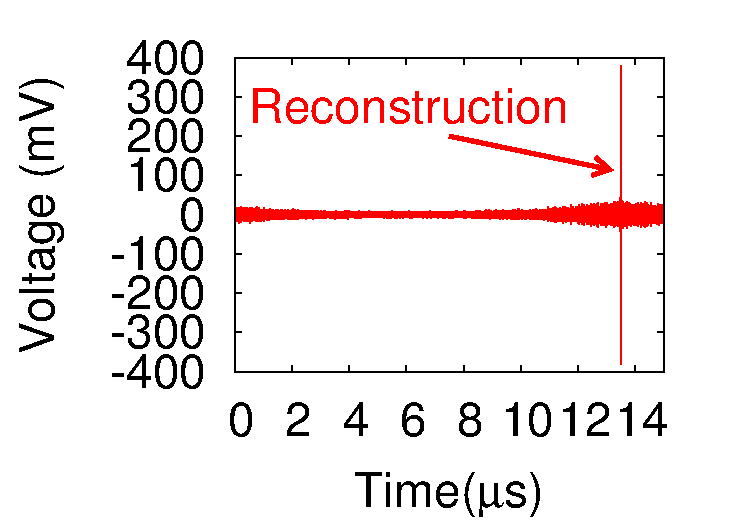
\includegraphics[width=\columnwidth,valign=t]{figs/recon.pdf}
				\caption{\label{fig:recon}}
		\end{subfigure}
	\end{subfigure}
  \vspace{-1\baselineskip}
	\caption{(a): A ray-chaotic enclosure with two antennas, one of
	which is attached to a sliding panel that can move freely along the $y$-axis,
	as shown in the right inset. A time-reversed sona (b) is broadcast from the
	transmitting antenna, resulting in a reconstruction at the receiving
	antenna, shown in (c).}
	\label{fig:setup}
\vspace{-0.5\baselineskip}
\end{figure}


\subsection{Experimental Setup}

We have investigated the applicability of time reversal to wireless power
transfer within an enclosed, reflective cavity (Fig.~\ref{fig:gigabox}): a
1.06~$m^3$ aluminum box with a conductive scattering paddle to make the ray
trajectories more ergodic.
%
Ray chaos ensures that a propagating pulse will eventually reach every point in
the environment, which insures that many transmission channels are
simultaneously excited, and this improves reconstruction fidelity.
%
The basic time reversal process in this environment proceeds as follows: First,
a 50~ns Gaussian pulse (with a carrier frequency of 5~GHz) is injected into
the cavity through the transmitting antenna.
%
A complex signal (referred to as a ``sona'') is measured at the receiving
antenna (Fig.~\ref{fig:sona}).
%
This sona is the sum of the reflections of the initial pulse, scaled in
magnitude due to ray-divergence and loss, and shifted in time due to differing
lengths of reflection paths.
%
In the next step, this sona is time reversed and injected into the transmitting
antenna.
%
The result is a reconstruction of the initial pulse back at the receiving
antenna (Fig.~\ref{fig:recon}).
%
This process makes use of another robust symmetry, namely the spatial
reciprocity of the wave equation.



Two monopole antennas inject and extract electromagnetic signals from different
points in the enclosure. A transmitting antenna is attached to the cavity wall
opposite the receiving antenna.
%
The receiving antenna is attached to a panel that can move vertically with a
total range of 70~mm.
%
Motion of the receiving antenna is achieved using an externally-mounted PI
MikroMove \texttt{M-415.DG} translation stage and the enclosure remains sealed
during the translation.



Interrogation pulses and time-reversed sona signals are created and broadcast
using a \texttt{Tektronix AWG7052} arbitrary waveform generator feeding an
\texttt{Agilent E8267D} Vector PSG microwave source.
%
A digital storage oscilloscope (DSO, \texttt{Agilent DSO91304A}) is used to
record waveforms of interest. MATLAB is used for signal processing and
instrument control and coordination.
%%%%%%%%%%%%%%%%%%%%%%%%%%%%%%%%%%%%%%%%%%%%%%%%%%%%%%%%%%%%%%%%%%%%%%%%%%%%%%%%
